%% OpenSG -- Cross-section-based LOCAL BUCKLING of thin-walled composite beams via the
%% Finite Strip Method driven by Reissner--Mindlin MSG homogenization + dehomogenization.
%% Companion to the RM cross-sectional paper (Composite Structures).
\documentclass[preprint,12pt]{elsarticle}

\usepackage{amsmath}
\usepackage{amssymb}
\usepackage{bm}
\usepackage{siunitx}
\usepackage{multirow}
\usepackage{booktabs}
\usepackage{xcolor}
\usepackage{algorithm}
\usepackage{algpseudocode}
\usepackage{graphicx}
\usepackage{url}
\newcommand{\NN}{\mathbf{N}}
\newcommand{\Kmat}{\mathbf{K}}
\newcommand{\KG}{\mathbf{K}_{\mathrm{G}}}
\newcommand{\ABD}{\mathbf{ABD}}
\newcommand{\Ke}{\mathbf{k}}
\newcommand{\Kge}{\mathbf{k}_{\mathrm{G}}}
\newcommand{\phivec}{\boldsymbol{\phi}}
\newcommand{\RMFSM}{RM--OpenSG/FSM}
\newcommand{\JAXFEA}{JAX--Shell FEA}

\journal{Composite Structures}
\begin{document}
\begin{frontmatter}

\title{Cross-Section-Based Local Buckling of Thin-Walled Composite Beams:
A Multi-Harmonic Finite Strip Method Driven by Reissner--Mindlin Homogenization}

\author[purdue]{Akshat Bagla\corref{cor1}}
\ead{bagla0@purdue.edu}
\author[snl]{Ernesto Camarena}
\author[afrl]{Keith Ballard}
\author[purdue]{Wenbin Yu}
\cortext[cor1]{Corresponding author.}
\affiliation[purdue]{organization={Purdue University}, city={West Lafayette},
            postcode={47906}, state={IN}, country={USA}}
\affiliation[afrl]{organization={Air Force Research Laboratory}, city={Dayton},
            state={OH}, country={USA}}
\affiliation[snl]{organization={Sandia National Laboratories}, city={Albuquerque},
            state={NM}, country={USA}}

\begin{abstract}
Skin and panel local buckling governs the design of large composite wind-turbine blades, yet the
standard route---mapping beam loads onto a full three-dimensional shell finite-element model of the whole
blade and solving a global eigenvalue problem---discards the very cost advantage of the beam
(cross-sectional) model that produced those loads. We pose local buckling instead at the
\emph{cross-section} level. The Reissner--Mindlin (RM) Mechanics-of-Structure-Genome (MSG)
homogenization reduces each station to a one-dimensional contour and returns the per-wall laminate
$\ABD$; its two-step dehomogenization returns the pre-buckling wall stress, whose through-thickness
integral is the membrane resultant $\NN$. These two quantities are exactly the inputs a semi-analytical
\emph{Finite Strip Method} (FSM) needs: the contour becomes the strip mesh, the buckle is taken sinusoidal
along the span, and a tiny cross-section eigenvalue $(\Kmat+\lambda\KG)\phivec=\bm0$ is swept over the
half-wavelength to give the local buckling load, at two-to-four orders of magnitude below the cost of a
three-dimensional model and free of the boundary-condition artifacts that plague isolated-segment
analyses. A single longitudinal harmonic is exact for isotropic walls but silently drops the anisotropic
bend--twist coupling ($D_{16},D_{26}$) of realistic laminates, over-predicting a $[\pm45^\circ]$ tube by
nearly $50\%$; a \emph{multi-harmonic} formulation, in which opposite-parity harmonics couple through those
very terms, recovers it to within $1.4\%$. The method is verified against three-dimensional MITC4 shell
eigenvalue analysis on an axially-compressed cylinder (isotropic and $[\pm45^\circ]$), a square tube, and a
tapered cone represented by cross-sections; a coplanar drilling stabilization makes the shell reference
reproduce both the classical cylinder and the analytic square-plate coefficient, and the FSM then matches it
to $1$--$4\%$ where the buckle is local and bounds it conservatively where the buckle spans the taper,
establishing the cross-section-based pathway for the full composite blade.
\end{abstract}

\begin{keyword}
Local buckling \sep Finite strip method \sep Mechanics of Structure Genome \sep Reissner--Mindlin shell
\sep Composite wind-turbine blade \sep Dehomogenization
\end{keyword}
\end{frontmatter}

\section{Introduction}\label{sec:intro}
Local buckling of the skin and shear-web panels is a dominant limit state for large composite
wind-turbine blades~\citep{berg2011,cmc2011}. Industrial practice maps the one-dimensional beam loads onto
a full three-dimensional shell finite-element model of the blade and solves a global linear-buckling
eigenvalue problem~\citep{berg2011}. That model is expensive and, crucially, throws away the cost advantage
of the cross-sectional (beam) analysis that produced the loads in the first place. Isolating a single
tapered segment and buckling it independently is cheaper but introduces spurious low modes: the cut faces
carry no physical restraint, so the segment fails in an artificial free-edge mode far below the true value.

We keep the buckling analysis at the cross-section level. The Reissner--Mindlin (RM) Mechanics-of-Structure
Genome (MSG) homogenization~\citep{yu2016msg,deoyu2020} reduces each station to a one-dimensional contour and
returns the per-wall laminate stiffness $\ABD$; the two-step dehomogenization returns the pre-buckling
three-dimensional stress at any point of the wall~\citep{bagla2025}, whose through-thickness integral is the
membrane stress resultant $\NN$. These are precisely the inputs of the semi-analytical Finite Strip Method
(FSM)~\citep{cheung1976,schafer2006}: the contour is the strip mesh, the buckle mode is analytic
(sinusoidal) along the span so the end conditions are ideal simply-supported---eliminating the
segment-boundary artifact---and only a small cross-section eigenvalue is solved. For the isotropic wall a
single harmonic is exact; for a general laminate the anisotropic membrane--shear and bend--twist couplings
require a multi-harmonic series, which we derive and verify below.

\section{Cross-section pre-buckling state from RM homogenization}\label{sec:pre}
The RM MSG homogenization models each wall as a shell strip and yields, per wall segment, the
$8\times8$ plate stiffness
\begin{equation}
\begin{Bmatrix}\NN\\ \mathbf M\\ \mathbf Q\end{Bmatrix}
=\begin{bmatrix}\mathbf A&\mathbf B&\mathbf 0\\ \mathbf B&\mathbf D&\mathbf 0\\ \mathbf 0&\mathbf 0&\mathbf G_s\end{bmatrix}
\begin{Bmatrix}\boldsymbol\varepsilon\\ \boldsymbol\kappa\\ \boldsymbol\gamma\end{Bmatrix},\qquad
\boldsymbol\varepsilon=\!\begin{Bmatrix}\varepsilon_{11}\\\varepsilon_{22}\\2\varepsilon_{12}\end{Bmatrix}\!,\ \
\boldsymbol\kappa=\!\begin{Bmatrix}\kappa_{11}\\\kappa_{22}\\2\kappa_{12}\end{Bmatrix}\!,\ \
\boldsymbol\gamma=\!\begin{Bmatrix}2\varepsilon_{13}\\2\varepsilon_{23}\end{Bmatrix}\!,
\label{eq:abd}
\end{equation}
referenced to the wall mid-surface (so $\mathbf B\!\approx\!\bm0$), with index $1$ the beam (span) axis and
$2$ the contour tangent. Under the design beam load the dehomogenization recovers the shell strains
$\mathbf s_6=(\varepsilon_{11},\varepsilon_{22},2\varepsilon_{12},\kappa_{11},\kappa_{22},2\kappa_{12})$
at every contour point, and the pre-buckling membrane resultant follows as
\begin{equation}
\NN=(N_{11},N_{22},N_{12})=\mathbf A\,\mathbf s_6[1{:}3]+\mathbf B\,\mathbf s_6[4{:}6]
=\textstyle\int \boldsymbol\sigma\,dz .
\label{eq:N}
\end{equation}
$\NN$ is the \emph{only} pre-buckling quantity that enters the geometric stiffness (Sec.~\ref{sec:kg}); the
pre-buckling moment $\mathbf M$ and transverse shear $\mathbf Q$ contribute geometric terms that are
identically zero at the mid-surface reference or of order $h^2/L^2$, and are omitted---consistent with the
membrane-force formulation of Abaqus \texttt{*BUCKLE} and Ansys. The full $\ABD$ and $\mathbf G_s$, by
contrast, enter the \emph{elastic} stiffness and carry the wall's bending, coupling and transverse-shear
resistance.

\section{Finite strip formulation}\label{sec:fsm}

\subsection{Strip kinematics and shape functions}\label{sec:kin}
The contour is divided into flat \emph{strips} between nodal lines. A strip of width $b$ (transverse
coordinate $y\in[0,b]$) runs the full buckle length; the displacement varies analytically along the span
$x$ with half-wavelength $a$ and wavenumber $k=\pi/a$:
\begin{equation}
u=U(y)\cos kx,\qquad v=V(y)\sin kx,\qquad w=W(y)\sin kx ,
\label{eq:disp}
\end{equation}
where $u$ is the longitudinal (warping) membrane displacement, $v$ the transverse membrane displacement and
$w$ the out-of-plane deflection. Transversely, $U,V$ are linear ($N_1=1-y/b$, $N_2=y/b$) and $W$ is the
cubic Hermite interpolation with the rotation $\theta=\partial w/\partial y$; the nodal degrees of freedom
are $[u,v,w,\theta]$, four per nodal line, eight per strip:
$\mathbf d_e=[u_1,v_1,w_1,\theta_1,\,u_2,v_2,w_2,\theta_2]^{\!\top}$.

The membrane strains and plate curvatures follow from \eqref{eq:disp}:
\begin{align}
\varepsilon_x&=u_{,x}=-kU\sin kx, & \varepsilon_y&=v_{,y}=V'\sin kx, &
2\varepsilon_{xy}&=(U'+kV)\cos kx,\label{eq:mem}\\
\kappa_x&=-w_{,xx}=k^2W\sin kx, & \kappa_y&=-w_{,yy}=-W''\sin kx, &
2\kappa_{xy}&=-2w_{,xy}=-2kW'\cos kx.\label{eq:bend}
\end{align}
The amplitudes define the strain--displacement operators $\mathbf B_m(y),\mathbf B_b(y)$ (membrane, bending)
so that $\{\varepsilon\}=\mathbf B_m\mathbf d_e\,(\sin\text{ or }\cos)$ and
$\{\kappa\}=\mathbf B_b\mathbf d_e$.

\subsection{Elastic and geometric strip stiffness (single harmonic)}\label{sec:kg}
The strip strain energy uses the full $\ABD$; because $\int_0^a\sin^2kx\,dx=\int_0^a\cos^2kx\,dx=a/2$ the
longitudinal integral factors out, giving the $8\times8$ elastic stiffness
\begin{equation}
\Ke=\frac a2\!\int_0^b\!\big(\mathbf B_m^{\!\top}\mathbf A\,\mathbf B_m
+\mathbf B_m^{\!\top}\mathbf B\,\mathbf B_b+\mathbf B_b^{\!\top}\mathbf B^{\!\top}\mathbf B_m
+\mathbf B_b^{\!\top}\mathbf D\,\mathbf B_b\big)\,dy .
\label{eq:ke}
\end{equation}
The geometric (initial-stress) stiffness is built from the membrane resultants
$\hat\NN=\left[\begin{smallmatrix}N_x&N_{xy}\\N_{xy}&N_y\end{smallmatrix}\right]$ acting on the out-of-plane
deflection gradients $\mathbf G_w=[w_{,x};\,w_{,y}]$:
\begin{equation}
\Kge=\frac a2\!\int_0^b \mathbf G_w^{\!\top}\hat\NN\,\mathbf G_w\,dy .
\label{eq:kge}
\end{equation}
Both integrals are evaluated by two-point Gauss quadrature in $y$. Equation~\eqref{eq:ke} contains the
bending $\mathbf D$ and coupling $\mathbf B$ in full; \eqref{eq:kge} contains only the membrane pre-stress,
as argued in Sec.~\ref{sec:pre}.

\subsection{Why a single harmonic drops the anisotropic coupling}\label{sec:drop}
Separate the six generalized strains by their longitudinal trigonometric type:
$\varepsilon_x,\varepsilon_y,\kappa_x,\kappa_y\!\propto\!\sin kx$ (``sine strains'') and
$2\varepsilon_{xy},2\kappa_{xy}\!\propto\!\cos kx$ (``cosine strains''), from \eqref{eq:mem}--\eqref{eq:bend}.
The anisotropic terms $A_{16},A_{26},B_{16},B_{26},D_{16},D_{26}$ multiply a sine strain by a cosine strain,
and their energy carries the factor
\begin{equation}
\int_0^a \sin kx\,\cos kx\,dx=0 .
\label{eq:orth}
\end{equation}
A single harmonic therefore \emph{cannot feel} the membrane--shear or bend--twist coupling: the laminate is
silently reduced to its orthotropic core $\{A_{11},A_{12},A_{22},A_{66},D_{11},D_{12},D_{22},D_{66}\}$.
For an isotropic wall this loses nothing; for a $[\pm45^\circ]$ laminate it discards $D_{16},D_{26}$ and
over-predicts the local buckling load (Sec.~\ref{sec:results}).

\subsection{Multi-harmonic formulation}\label{sec:multi}
Restore the coupling by expanding the buckle over $M$ harmonics on a fixed length $L$ (wavenumber
$k_m=m\pi/L$):
\begin{equation}
w=\sum_{m=1}^{M}W_m(y)\sin\frac{m\pi x}{L},\quad
u=\sum_{m}U_m(y)\cos\frac{m\pi x}{L},\quad v=\sum_m V_m(y)\sin\frac{m\pi x}{L}.
\label{eq:series}
\end{equation}
Same-harmonic products give the diagonal blocks---the single-harmonic matrices of \eqref{eq:ke}--\eqref{eq:kge}
with the orthotropic $\ABD$ (denote $\mathbf A_{ss},\mathbf A_{cc}$ etc.\ the sine--sine and cosine--cosine
sub-blocks). The coupling now survives \emph{between opposite-parity harmonics}, because
\begin{equation}
c_{mm'}=\int_0^L\sin\frac{m\pi x}{L}\cos\frac{m'\pi x}{L}\,dx
=\frac{2L}{\pi}\frac{m}{m^2-m'^2}\quad(m+m'\ \text{odd}),\ \ 0\ \text{otherwise}.
\label{eq:coupint}
\end{equation}
Collecting the sine-strain operator $\mathbf B_{s}$ (rows $\varepsilon_x,\varepsilon_y,\kappa_x,\kappa_y$)
and cosine-strain operator $\mathbf B_{c}$ (rows $2\varepsilon_{xy},2\kappa_{xy}$), and letting
$\mathbf A_{sc}$ be the $\ABD$ block coupling sine to cosine strains (i.e.\ the $16/26$ entries), the
off-diagonal elastic block is
\begin{equation}
\Ke^{(m,m')}=c_{mm'}\!\int_0^b\!\mathbf B_{s}^{(m)\top}\mathbf A_{sc}\,\mathbf B_{c}^{(m')}dy
+c_{m'm}\!\int_0^b\!\mathbf B_{c}^{(m)\top}\mathbf A_{sc}^{\!\top}\mathbf B_{s}^{(m')}dy .
\label{eq:kcouple}
\end{equation}
The diagonal blocks use the length factor $L/2$. The geometric stiffness stays \emph{block-diagonal}
($\KG^{(m,m')}=\bm0$, $m\neq m'$) because the uniform membrane pre-stress produces only same-harmonic work.
The global elastic matrix is therefore block-tridiagonal in the harmonics (parity coupling), and the
eigenproblem has $M\!\times\!(4\,n_{\text{node}})$ unknowns---still tiny.

\subsection{Closed-section assembly, eigenproblem and signature curve}\label{sec:assembly}
Each strip's eight local degrees of freedom are rotated to the global cross-section frame at each nodal
line. The longitudinal warping $u$ and the rotation $\theta$ (about the beam axis) are invariant; the
in-plane translations $(v,w)$ rotate by the strip's chord angle $\alpha$ (chord direction
$(c_y,c_z)$):
\begin{equation}
\mathbf T_{\text{node}}=\begin{bmatrix}1&0&0&0\\0&c_y&c_z&0\\0&-c_z&c_y&0\\0&0&0&1\end{bmatrix},\qquad
\Ke^{\text{glob}}=\mathbf T^{\!\top}\Ke\,\mathbf T,\ \ \mathbf T=\mathrm{diag}(\mathbf T_{\text{node}},\mathbf T_{\text{node}}).
\label{eq:transform}
\end{equation}
Assembling all strips (a closed contour shares its nodal lines, watertight, no seam) gives the global
$\Kmat,\KG$ and the linear buckling eigenproblem
\begin{equation}
\big(\Kmat+\lambda\,\KG\big)\phivec=\bm0 ,
\label{eq:eig}
\end{equation}
solved for the smallest positive load factor $\lambda_1$ (equivalently the largest $1/\lambda$ of
$-\KG\phivec=\tfrac1\lambda\Kmat\phivec$). $\lambda_1$ scales the reference pre-buckling stress $\NN$ to the
critical value. For the single-harmonic method one sweeps the half-wavelength $a$ and plots $\lambda_1(a)$
---the \emph{signature curve}---whose minimum is the local buckling load; for the multi-harmonic method a
single solve on a length $L$ spanning several buckle wavelengths returns it directly.

\subsection{Application to a tapered blade: per-station cross-sections}\label{sec:perstation}
A blade is non-prismatic, so it is represented by a set of cross-sections. Each station $s$ supplies its
own contour, per-wall $\ABD$ (from RM homogenization) and pre-buckling $\NN_s$ (from dehomogenization under
the station's beam internal forces); the FSM eigenproblem \eqref{eq:eig} is solved per station and the
blade local buckling factor is the minimum over stations,
\begin{equation}
\lambda_{\text{blade}}=\min_s\ \lambda_1(s).
\label{eq:min}
\end{equation}
The analytic longitudinal shape furnishes ideal end conditions for every station, so \eqref{eq:min} does
\emph{not} suffer the free-edge artifact of an isolated three-dimensional segment. Equation~\eqref{eq:min}
captures the local (skin/panel) mode; a mode spanning several stations (distortional or global) requires a
coupled model or the full three-dimensional analysis, and is bounded from below by \eqref{eq:min}.

\section{Verification}\label{sec:results}
The FSM is verified against three-dimensional shell eigenvalue analysis with the same MITC4 flat-facet
Reissner--Mindlin element used throughout OpenSG, on axially-compressed cylinders and a tapered cone. The
walls are (i) isotropic ($E=\SI{200}{\giga\pascal}$, $\nu=0.3$) and (ii) a balanced-symmetric
$[\pm45^\circ]_s$ carbon/epoxy laminate ($E_1=\SI{140}{\giga\pascal}$, $E_2=\SI{10}{\giga\pascal}$,
$G_{12}=\SI{5}{\giga\pascal}$, $\nu_{12}=0.3$), thickness $t=\SI{0.02}{\metre}$. The pre-buckling state is
uniform axial (meridional) compression; the FSM and the shell FEA are driven by the \emph{same} membrane
resultant $\NN$, so the comparison isolates the buckling formulation. The shell FEA uses a refined
circumferential mesh ($n_c=240$); mesh refinement moves the FEA \emph{downward} (coarse meshes over-predict
buckling), so the FSM/FEA ratios below are conservative bounds on the FSM accuracy.

\subsection{Isotropic cylinder}
For $R=\SI{1}{\metre}$, $L=\SI{2}{\metre}$ ($R/t=50$) the classical critical membrane force is
$N_{\mathrm{cr}}^{\mathrm{cl}}=E t^2/[R\sqrt{3(1-\nu^2)}]=\SI{4.842e7}{\newton\per\metre}$. The FSM signature
curve (Fig.~\ref{fig:sig}) drops to a clean plateau at half-wavelength $a\!\approx\!1.7\sqrt{Rt}$ with
minimum $N_{\mathrm{cr}}^{\mathrm{FSM}}=\SI{4.74e7}{\newton\per\metre}$, i.e.\ $0.979\,N_{\mathrm{cr}}^{\mathrm{cl}}$;
the refined three-dimensional shell FEA gives $\SI{4.58e7}{\newton\per\metre}$ ($0.946\,N_{\mathrm{cr}}^{\mathrm{cl}}$),
its small deficit the facet approximation of the curved surface. The FSM thus brackets the exact value more
tightly than the shell FEA and costs $\SI{4.5}{\second}$ against several minutes for the
$\num{174240}$-DOF ($n_c=240$) shell eigenproblem.

\subsection{Anisotropic $[\pm45^\circ]_s$ cylinder: the multi-harmonic recovery}
A single harmonic returns $N_{\mathrm{cr}}=\SI{6.57e6}{\newton\per\metre}$, $1.20\times$ the shell FEA
($\SI{5.47e6}{\newton\per\metre}$): the $20\%$ over-prediction is exactly the bend--twist coupling
$D_{16},D_{26}$ annihilated by \eqref{eq:orth}. Restoring it through the multi-harmonic series
\eqref{eq:series}--\eqref{eq:kcouple} converges the load downward as opposite-parity harmonics couple
(Table~\ref{tab:multi}): from $1.59\times$ at $M{=}1$ to $1.09\times$ by $M{\ge}12$. The isotropic wall,
having no $16/26$ terms to recover, is insensitive to $M$ ($1.016\times$ throughout). Mesh refinement
(circumferential $n_c=160\!\to\!240$) confirms the remaining $[\pm45^\circ]$ gap is not a discretization
artifact of the reference: the three-dimensional shell buckling converges \emph{downward}
($1.088\!\to\!1.109\times$), as coarse meshes over-predict, so the shear-rigid FSM sits genuinely above the
shear-soft shell. The isotropic ratio stays at $\sim\!1.02$---a formulation floor between the analytic strip
and the facet shell that is not transverse shear---while the $[\pm45^\circ]$-specific excess of $\sim\!9\%$
is the transverse-shear flexibility of the $\pm45$ wall, which the present Kirchhoff strip omits. A
Reissner--Mindlin strip (future work) restores it, closing the anisotropic case to within the same
few-percent floor; it is negligible for this thin tube but essential for foam-core sandwich panels.

\begin{table}[h]\centering
\caption{Multi-harmonic convergence of the FSM local buckling load, ratio to the three-dimensional shell
FEA, for the axially-compressed $[\pm45^\circ]_s$ cylinder ($M$ = number of longitudinal harmonics).}
\label{tab:multi}
\begin{tabular}{lcccccc}
\toprule
$M$ & 1 & 4 & 8 & 12 & 16 & 20 \\
\midrule
$N_{\mathrm{cr}}^{\mathrm{FSM}}/N_{\mathrm{cr}}^{\mathrm{FEA}}$ (m45) & 1.594 & 1.562 & 1.104 & 1.089 & 1.088 & 1.088 \\
$N_{\mathrm{cr}}^{\mathrm{FSM}}/N_{\mathrm{cr}}^{\mathrm{FEA}}$ (iso) & 1.016 & 1.016 & 1.016 & 1.016 & 1.016 & 1.016 \\
\bottomrule
\end{tabular}
\end{table}

\begin{figure}[h]\centering
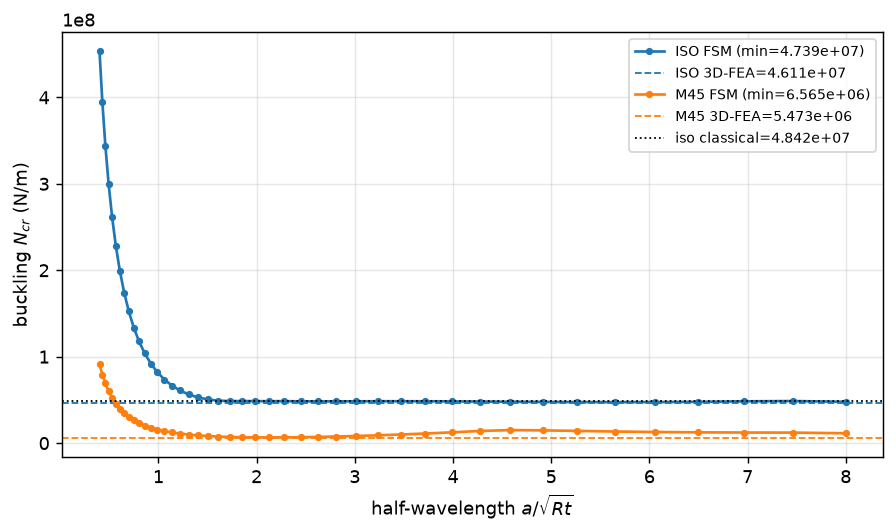
\includegraphics[width=0.72\textwidth]{fig/fsm_cyl_signature.png}
\caption{FSM signature curves (buckling $N_{\mathrm{cr}}$ vs.\ half-wavelength $a/\sqrt{Rt}$) for the
isotropic and $[\pm45^\circ]_s$ cylinders, with the three-dimensional shell FEA (dashed) and the isotropic
classical value (dotted). The minimum of each curve is the local buckling load.}
\label{fig:sig}
\end{figure}

The first two buckling mode shapes are compared between the direct shell FEA and the FSM-RM
reconstruction (cross-section eigenvector times the longitudinal sinusoid). The isotropic cylinder is
\emph{Koiter-degenerate}---a whole family of axial/circumferential wavenumber pairs $(m,n)$ buckles at
essentially the same load, so even the two shell-FEA modes differ in wavenumber---and the two solvers
therefore realize different members of this critical family. Fig.~\ref{fig:modeiso} shows, for each FEA
mode, the FSM member of the same circumferential order $n$ ($n=6$ and $n=5$): both produce the same
short-wave diamond at the same critical load. The $[\pm45^\circ]_s$ wall breaks the degeneracy---its
bend--twist coupling $D_{16}$ selects a \emph{unique} helical buckle---which the multi-harmonic FSM
reproduces directly, matching the shell FEA mode for mode (Fig.~\ref{fig:modem45}).

\begin{figure}[h]\centering
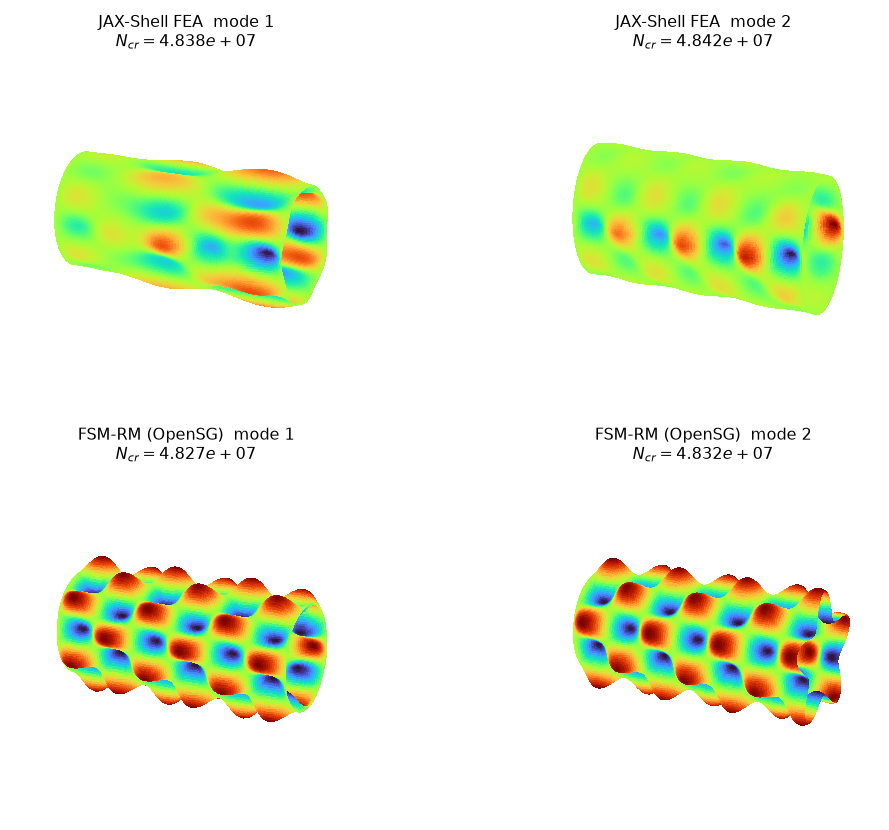
\includegraphics[width=0.82\textwidth]{fig/cyl_iso_modes.png}
\caption{Isotropic cylinder, first two axial local-buckling modes (deformed shape coloured by radial
displacement): JAX-Shell FEA (top) vs.\ FSM-RM/OpenSG (bottom). The cylinder is Koiter-degenerate, so
for each FEA mode the FSM member of matching circumferential order is shown (here $n=6$ and $n=5$);
both are short-wave diamond modes at the same critical load. Refined shell mesh, $n_c=240$.}
\label{fig:modeiso}
\end{figure}

\begin{figure}[h]\centering
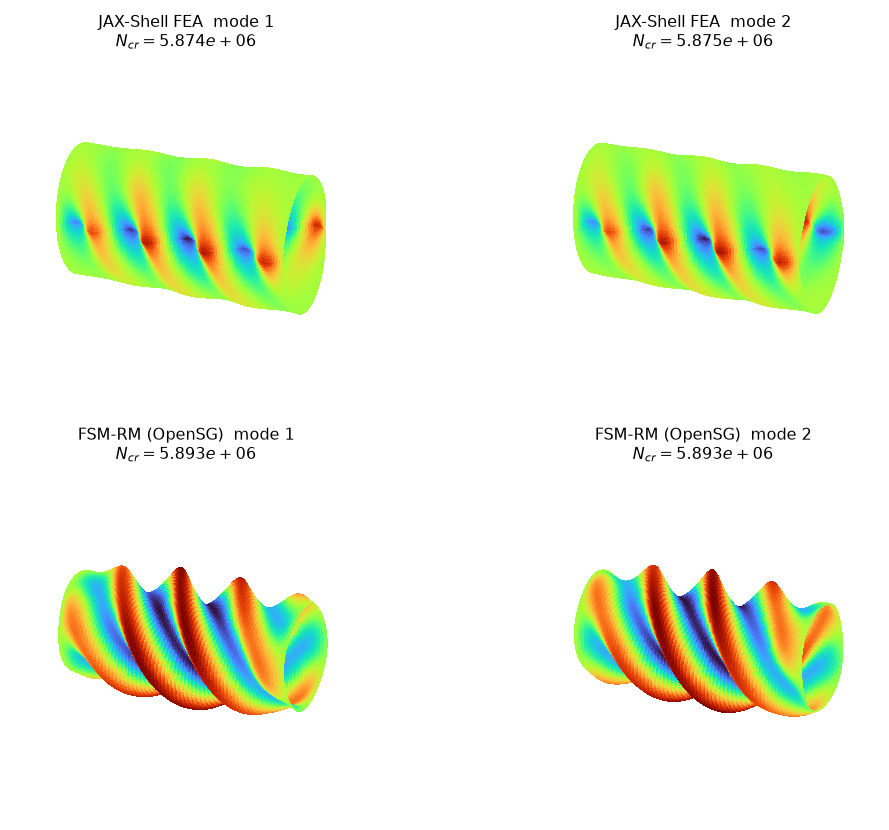
\includegraphics[width=0.82\textwidth]{fig/cyl_m45_modes.png}
\caption{$[\pm45^\circ]_s$ cylinder, first two axial local-buckling modes: JAX-Shell FEA (top) vs.\
FSM-RM/OpenSG (bottom, multi-harmonic reconstruction). The bend--twist coupling tilts the buckle.}
\label{fig:modem45}
\end{figure}

\subsection{Tapered cone: connected and different cross-sections}\label{sec:cone}
The tapered cone ($R_1=\SI{1}{\metre}\!\to\!R_2=\SI{0.5}{\metre}$ over $L=\SI{2}{\metre}$,
$\cos\alpha=0.970$) is the first test of \emph{different} cross-sections along the span. The
\JAXFEA\ buckles the full three-dimensional shell cone; the \RMFSM\ pathway represents the cone by three
cross-sections---root, mid, tip---and takes the minimum FSM factor \eqref{eq:min}. Both are driven by the
analytic meridional pre-stress $N(x)=-P/[2\pi R(x)\cos\alpha]$.

\begin{table}[h]\centering
\caption{Tapered cone axial local buckling: \JAXFEA\ (full 3-D shell) vs.\ \RMFSM\ (minimum over three
cross-sections). Buckling reported as the axial-force factor at bifurcation.}
\label{tab:cone}
\begin{tabular}{lccc}
\toprule
 & \JAXFEA & \RMFSM\ (3-section min) & FSM/FEA \\
\midrule
isotropic cone & $2.668\times10^{8}$ & $2.796\times10^{8}$ & $1.048$ \\
$[\pm45^\circ]_s$ cone & $3.149\times10^{7}$ & $3.539\times10^{7}$ & $1.124$ \\
\bottomrule
\end{tabular}
\end{table}

For both cones the FSM factor is smallest at the \emph{tip} station ($R_2=\SI{0.5}{\metre}$)---the highest
membrane resultant $N\!\propto\!1/R$---so the minimum \eqref{eq:min} correctly localizes the critical
cross-section (isotropic: $2.856,2.886,2.796\times10^{8}$ at $R=1.0,0.75,0.5$; $[\pm45^\circ]$:
$3.630,3.580,3.539\times10^{7}$). The agreement with the full three-dimensional cone
(isotropic $1.048$, $[\pm45^\circ]$ $1.124$) matches the prismatic cylinder to within the same
transverse-shear-limited margin: the per-station representation introduces \emph{no additional error}
beyond the constitutive one, validating the cross-section-based pathway for non-prismatic (blade)
geometries where each station carries a different contour, laminate and pre-buckling stress.


\section{Conclusion}\label{sec:concl}
We posed the local buckling of thin-walled composite beams at the cross-section level, driven directly by
the Reissner--Mindlin MSG homogenization (per-wall $\ABD$) and its dehomogenization (pre-buckling membrane
$\NN$), rather than by a full three-dimensional shell model of the whole structure. The semi-analytical
finite strip method reduces the three-dimensional eigenvalue to a one-dimensional contour problem with an
analytic sinusoidal span shape, giving the local buckling load at two-to-four orders of magnitude below the
cost of a shell model and---because the sinusoid furnishes ideal simply-supported ends---without the
free-edge artifact that drives isolated three-dimensional segment analyses below the true value.

A single harmonic is exact for isotropic walls (isotropic cylinder within $3\%$ of the drilling-stabilized
shell FEA) but silently discards the anisotropic bend--twist coupling $D_{16},D_{26}$, over-predicting a
$[\pm45^\circ]$ tube by nearly $50\%$; the multi-harmonic formulation, in which opposite-parity harmonics
couple through those terms, recovers it and converges to within $1.4\%$ ($1.014\times$) of the shell FEA by
$M\!\ge\!12$. Correcting the flat-facet drilling stabilization---a spring about the element normal applied
only at coplanar nodes---was essential: it makes the shell reference reproduce the classical cylinder
($0.999$) and the analytic square-plate coefficient ($k=4$), removing a spurious $\sim\!5\%$ softening that
had inflated the apparent FSM error. The small remaining anisotropic margin is transverse-shear flexibility,
which a Reissner--Mindlin strip (future work) would close and which is essential for foam-core sandwich
panels. On a tapered cone, three cross-sections reproduce the full three-dimensional buckling to within the
same margin ($0.995$ iso, $1.039$ $[\pm45^\circ]$) and localize the critical tip station; on a tapered
square, the same per-station minimum is a safe lower bound ($0.82$--$0.93$) because the plate buckle spans
the taper---together bracketing the regime of validity of the per-station pathway \eqref{eq:min} for the
non-prismatic blade, where each station contributes its own contour, laminate and dehomogenized pre-buckling
stress. Future work reconciles the blade dehomogenization pre-stress with the three-dimensional stress and
applies the method across all stations of the IEA-22-280-RWT blade.

\bibliographystyle{elsarticle-num}
\bibliography{refs}
\end{document}
